%% Manuscript for the Journal of Healthcare Informatics Research (Springer).
%% English version. Template: Springer Nature sn-jnl, reference style sn-basic
%% (numbered brackets, entries of the form Author, A.A.: Title. Journal vol,
%% pages (year)).
%%
%% Build: upload this single .tex into an Overleaf project that already contains
%% sn-jnl.cls and the figure files, and compile with pdfLaTeX. References are
%% inline (thebibliography), no .bib file needed.
%%
%% Content mirrors Sadykhov_DKA_recurrence_RU.md (analytical sample of 314 patients).

\documentclass[pdflatex,sn-basic,Numbered]{sn-jnl}

%%%% Standard template packages
\usepackage{graphicx}%
\usepackage{multirow}%
\usepackage{amsmath,amssymb,amsfonts}%
\usepackage{amsthm}%
\usepackage[title]{appendix}%
\usepackage{xcolor}%
\usepackage{textcomp}%
\usepackage{manyfoot}%
\usepackage{booktabs}%

\raggedbottom

\begin{document}

\title[Clinical Factors of Recurrent DKA]{Clinical Factors of Recurrent Diabetic Ketoacidosis: An Analysis of a Russian Cohort Using Statistics and Interpretable Machine Learning}

\author*[1]{\fnm{Oleg} \sur{Sadykhov}}\email{ovelsad@niuitmo.ru}

\author[1]{\fnm{Vasiliy} \sur{Leonenko}}\email{vnleonenko@itmo.ru}

\affil*[1]{\orgdiv{Artificial Intelligence Technologies Faculty}, \orgname{ITMO University}, \orgaddress{\street{49 Kronverksky Pr.}, \city{St. Petersburg}, \postcode{197101}, \country{Russia}}}

\abstract{\textbf{Purpose.} To identify clinical factors associated with a recurrent course of diabetic ketoacidosis (DKA) in a Russian cohort and to assess, using interpretable machine learning, how far these groups differ in clinical profile at admission.

\textbf{Methods.} A retrospective single-center study, predictors and outcome refer to the same hospitalization. Time to event was not recorded, so the model is diagnostic rather than prognostic. The outcome was established in 314 patients (recurrent course 101, single episode 213). Groups were compared under a fixed statistical protocol with Benjamini-Hochberg correction. Independently, five interpretable models were fitted (logistic regression, random forest, and gradient boosting in three implementations, XGBoost, LightGBM, CatBoost) on 25 outcome-independent features without multicollinearity, the split preceding preprocessing and hyperparameters tuned by nested cross-validation. Feature contributions were estimated by SHAP and compared with the statistics. One hypothesis was pre-specified, on the association of alcohol intake with a recurrent course.

\textbf{Results.} A recurrent course was distinguished by a longer diabetes duration, a median of 9.0 against 6.75 years, a higher daily insulin dose and a higher HDL cholesterol, at a lower HbA1c, 11.0 against 12.2\%. Chronic kidney disease, retinopathy and diabetic neuropathy were more frequent in the recurrent group. The alcohol hypothesis was confirmed, alcohol intake in the day before a DKA episode raised the odds of a recurrent course, OR 2.01 (95\% CI 1.14-3.56). The five models showed close and moderate discrimination, ROC-AUC 0.67-0.73 by nested cross-validation and 0.65-0.76 on the held-out test. Gradient boosting was ahead in point estimates, logistic regression weaker. Pairwise comparison of the areas under the curve by the DeLong test with correction revealed no significant differences. By SHAP the gradient boosting models consistently highlighted daily insulin dose, HbA1c, diabetes duration, insulin delivery method and glucose at admission. The leading model XGBoost, at the Youden operating point, identified 80\% of recurrences on the held-out test at a specificity of 0.58, against 65\% at the neutral threshold of 0.5.

\textbf{Conclusion.} In a Russian cohort of 314 patients, a recurrent course of DKA is associated with a longer diabetes duration, a higher daily insulin dose, alcohol intake, and renal and microvascular complications. Interpretable models separate the groups moderately, ROC-AUC about 0.7, gradient boosting ahead in point estimates, but statistically no model outperforms the others. The modest metrics and single-center data call for validation on external data before clinical use.}

\keywords{diabetic ketoacidosis, recurrent course, risk factors, interpretable machine learning, SHAP, diagnostic model}

\maketitle

\section{Introduction}\label{sec1}

Diabetic ketoacidosis is a life-threatening complication of diabetes mellitus, characterized by hyperglycemia, metabolic acidosis and an elevated concentration of ketone bodies \cite{ref1}. Between 2003 and 2014 the United States recorded 1,760,101 primary DKA hospitalizations, and the number of discharges with a principal diagnosis rose from 118,808 in 2003 to 188,965 in 2014 \cite{ref2}. After the acute state is resolved, single cases may progress to repeated episodes, and a recurrent course carries substantially higher mortality \cite{ref3,ref4}.

Repeated DKA episodes are rarely explained by a single cause. Risk factors for repeated admissions include young age, psychiatric disorders, infections, non-adherence to therapy, alcohol and psychoactive substance abuse, and socioeconomic circumstances \cite{ref5,ref6,ref7}. The set of factors is heterogeneous, results across studies agree poorly, and for the Russian population the factors of a recurrent course have not been described. Despite decades of clinical experience, optimal DKA management strategies remain a subject of debate \cite{ref8}.

Closest to our task is a case-control observational study that matched patients with recurrent and single courses on age, diabetes duration, sex and ethnicity \cite{ref9}. After matching, few appreciable differences between the groups remained, and the main trigger of an episode in both groups was missed insulin injections. With 40 patient pairs such a result is hard to interpret unambiguously, it may mean either an absence of differences or a lack of power. The question of which patient characteristics are associated with a recurrent course remains open.

Machine learning allows the same task to be viewed from another angle. Published DKA models reach ROC-AUC of about 0.82-0.85 \cite{ref10,ref11}, but they address a different task, they predict the first episode or the fact of hospitalization within a set time window, they rely on large foreign electronic health record databases with a high proportion of missing values, and on other samples their metrics usually do not reproduce \cite{ref11}. It has also been shown \cite{ref12,ref13} that many models work as a black box, their conclusions are hard to interpret, which reduces clinicians' trust and becomes a barrier to adoption. Current work in diabetology applies prediction explanation methods, primarily SHAP and LIME \cite{ref14,ref15}, but for a recurrent course of DKA such tools have hardly been used.

In this work we identify the clinical factors associated with a recurrent course of DKA in a Russian cohort and assess how far a patient's clinical profile at admission can distinguish a recurrent course from a single episode. The key feature of the approach is that we obtain the set of factors along two independent paths, classical statistics under an agreed protocol and SHAP on top of interpretable machine learning models, after which we compare the results. Such a comparison shows to what extent the set of factors depends on the chosen analytical approach, which matters especially in a small sample.

The clinical hypothesis on the association of alcohol intake with a recurrent course was set before training. Alcohol is listed among the predisposing and precipitating factors of repeated DKA episodes \cite{ref7}, and the same association is described in studies of repeated admissions \cite{ref9,ref16}. Testing this association in a Russian cohort is the first task of the work. The second task is to build a diagnostic model of a recurrent course from the clinical profile at admission, for which five algorithms, from logistic regression to gradient boosting, were trained and then compared by the DeLong test, since in clinical prediction models machine learning did not outperform logistic regression \cite{ref17}.

\section{Methods}\label{sec2}

\subsection{Design and Data Source}\label{subsec2_1}

A retrospective single-center study on de-identified data with cross-sectional outcome ascertainment, both predictors and outcome refer to the same DKA hospitalization, with no observation period between them. The analysis included patients hospitalized with diabetic ketoacidosis between 2019 and 2026. Inclusion criteria were age 18 years or older and a confirmed diagnosis of DKA. The only exclusion criterion was an undetermined outcome. The initial sample comprised 330 patients, and the outcome was established in 314.

\subsection{Outcome}\label{subsec2_2}

The target variable was a recurrent course of DKA (0 for a single episode, 1 for a recurrent course). A patient was assigned to the recurrent group if more than one DKA episode had been recorded in total. The episode count combined the number of the patient's prior visits to this hospital with the same diagnosis from the medical records, the history at admission when the patient had not been observed here before, and the current hospitalization. A single course was defined as a first and only presentation.

The outcome was ascertained retrospectively, so at the time the predictors were measured it had in most cases already occurred. The data contain no fixed observation window, no dates of individual episodes and no time to event, and there is no censoring. Under the TRIPOD classification the model is diagnostic, it recognizes a state that has already occurred rather than predicting a future event. The task addressed is the separation of a recurrent from a single course by the patient's clinical profile and the identification of factors associated with it. The consequences for interpretation are discussed in the limitations section.

\subsection{Hypothesis}\label{subsec2_3}

The hypothesis was formulated in advance, before data analysis, on the basis of the literature. Clinical hypothesis. H0: alcohol intake in the day before an episode is not associated with a recurrent course (odds ratio equals 1). H1: an association exists (odds ratio differs from 1). Test, the protocol test for a 2$\times$2 table, effect measure, odds ratio with a 95\% confidence interval, with the Benjamini-Hochberg correction for multiple comparisons. We put forward no other hypotheses. The comparison of models by discrimination and all other statistical comparisons are descriptive, and features with significant differences between groups are treated as an exploratory result requiring confirmation on an independent sample.

\subsection{Predictors}\label{subsec2_4}

We used indicators collected at hospitalization, demographic data (age, sex), history and therapy of diabetes (type, duration, age at onset, insulin delivery method, daily dose), laboratory indicators at admission (blood gases, electrolytes, creatinine, urea, glucose, HbA1c, lipid panel), complications (chronic kidney disease by stage and albuminuria, diabetic retinopathy and polyneuropathy) and a lifestyle factor (alcohol intake).

The models were trained on a single feature set, 25 indicators without marked multicollinearity. Age is almost linearly related to age at onset and diabetes duration (Pearson correlation about 0.99), so age at onset was removed as linearly dependent. The composition of the set was determined only by the mutual correlation of predictors and did not depend on the outcome, so feature selection introduces no bias into the quality estimate.

\subsection{Sample Size}\label{subsec2_5}

The sample size was not calculated in advance, the study is retrospective, so all available observations entered the analysis, 314 patients with an established outcome (recurrent course proportion 32.2\%, 101 events). With 101 events for 25 features there are few observations of the rare class, which raises the risk of overfitting, so we limited dimensionality and applied regularization and class weighting. Signs of overfitting were sought in three ways, by comparing estimates on nested cross-validation and the held-out test, by the out-of-bag estimate of the random forest, and by 95\% confidence intervals of the metrics from bootstrap.

\subsection{Missing Data}\label{subsec2_6}

The proportion of missing values per indicator ranged from a few percent to 60\% (HbA1c, sodium, potassium, lactate), the full picture is shown in Fig.~\ref{figmiss}. We assumed the values were missing at random conditional on the observed variables, and accounted for their panel structure, where laboratory indicators go missing in groups. We compared imputation strategies, median and mode, k-nearest neighbors, and multiple imputation by chained equations. The imputer was trained only on the training part within folds, and on the test set missing values were filled from the nearest neighbors of the training part, without using the outcome or other test observations.

The working choice was k-nearest neighbors imputation with five neighbors. It outperformed the other strategies in model quality and did not appreciably distort the shape of the distributions, when comparing distributions before and after imputation by the Kolmogorov-Smirnov test no significant discrepancies were found. The number of neighbors was compared separately (k from 3 to 11) by out-of-fold ROC-AUC on the training part, and k = 5 proved best.

\subsection{Statistical Analysis}\label{subsec2_7}

Normality was tested by the Shapiro-Wilk test for n below 50 and by the Kolmogorov-Smirnov test in the Lilliefors variant for n of 50 or more. Quantitative indicators with a normal distribution were described by mean and standard deviation with a 95\% confidence interval, and when departing from normality by median and quartiles. Groups were compared by the Student t-test, the Mann-Whitney U test or the Brunner-Munzel test depending on normality and equality of variances (Levene test). Proportions in 2$\times$2 tables were compared by the Pearson chi-square test when the minimum expected frequency exceeded 10 and by the Fisher exact test when the expected frequency was below 10. The confidence interval for proportions was computed by the Clopper-Pearson method, and the effect size by the odds ratio with a 95\% confidence interval. For multiple comparisons the Benjamini-Hochberg correction was applied. Areas under the ROC curves of two models on the same patients were compared by the DeLong test for correlated curves.

\subsection{Model Development}\label{subsec2_8}

The sample was split once, stratified, in an 80 to 20 ratio, training part 251 patients, test 63. The split was performed before any preprocessing, with a fixed random seed. All preprocessing (imputation, scaling, encoding of categorical features, balancing) was performed inside the pipeline and trained only on the training folds.

The choice of strategies and model families was made entirely on the training part, the held-out test was not consulted at this stage. We compared seven families (logistic regression, random forest, LightGBM, CatBoost, XGBoost, support vector machine, k-nearest neighbors) along the axes of imputation, balancing, categorical encoding and transformation of quantitative features, the comparison criterion being out-of-fold ROC-AUC on the training part.

Five families were taken forward, logistic regression as a linear model, random forest as a bagging method, and XGBoost, LightGBM and CatBoost as gradient boosting variants, the last of which handles categorical features natively. The support vector machine and k-nearest neighbors were excluded for two reasons, their out-of-fold ROC-AUC was the lowest (0.672 and 0.639 against 0.679-0.720 for the others), and they do not provide the additive feature contributions required for the SHAP analysis central to this work.

Class imbalance was handled by class weighting, and synthetic methods (SMOTE, SMOTENC, BorderlineSMOTE, ADASYN) were compared separately. Hyperparameters were tuned by Bayesian search in nested cross-validation, the procedure quality was assessed by an outer five-fold cross-validation, while within each training fold the hyperparameters were tuned by a separate three-fold cross-validation.

\subsection{Performance Assessment}\label{subsec2_9}

Model quality was assessed by the area under the ROC curve (ROC-AUC) and under the precision-recall curve (PR-AUC), and for each we report a 95\% confidence interval from bootstrap (2000 replicates). These metrics show how far the clinical profile at admission separates the groups. Probability calibration was checked by out-of-fold calibration curves and the Brier score, comparing raw probabilities with the Platt and isotonic regression methods. The reduction of the Brier score was small, no more than 0.03, and inconsistent between models. Raw probabilities are therefore reported, and calibration is kept as an option for clinical deployment where an accurate absolute probability is needed.

We also report the confusion matrix at a chosen classification threshold. The main threshold, above which a prediction was assigned to a recurrent course, was chosen on the out-of-fold probabilities of the training part by the maximum of the Youden index, then fixed and applied once to the held-out test. The threshold at the maximum of F2, which shifts the balance toward recall, is reported additionally for comparison. To assess how far the threshold and the metrics at it depend on the sample composition, the training part was resampled by bootstrap with re-selection of the threshold, and confidence intervals were built. At this sample size the threshold changes noticeably from replicate to replicate, so we do not treat it as a clinical recommendation but choose it for subsequent work oriented toward clinical use.

\subsection{Interpretation}\label{subsec2_10}

Feature contributions were estimated by SHAP for all five models, LinearSHAP for logistic regression, TreeSHAP for random forest, XGBoost and LightGBM, and the built-in SHAP value computation for CatBoost. The contributions of one-hot encoded categories were summed back to the source feature, and feature importance was measured by the mean absolute SHAP value. Feature importance was examined at two levels. The first level is agreement among the models, assessed by the pairwise Spearman rank correlation between the full rankings. The stability of the rankings to the sample composition was checked by bootstrap, 200 replicates, in each the training part was resampled with replacement, all five models were refitted with fixed hyperparameters, SHAP was computed on the observations not drawn into the sample, and for each model we counted how often a feature enters the top-10. The second level is the comparison of machine learning with classical statistics, whether the features the models rank highly by SHAP coincide with the list of indicators significant in the between-group comparison.

\subsection{Software and Reporting}\label{subsec2_11}

The analysis was performed in Python 3.11 with fixed library versions, and the code is open. Reporting follows the STROBE recommendations for observational studies, and for the part concerning model development the TRIPOD+AI recommendations were additionally taken into account.

\section{Results}\label{sec3}

\subsection{Participant Characteristics}\label{subsec3_1}

Of the initial cohort of 330 patients, 16 without an established outcome were excluded (Fig.~\ref{figflow}). The analytical sample comprised 314 patients, 101 with a recurrent course (32.2\%) and 213 with a single episode. The stratified split gave a training part of 251 patients (81 with a recurrent course, 170 with a single episode) and a test part of 63 (20 and 43 respectively).

\begin{figure}[h]%
\centering
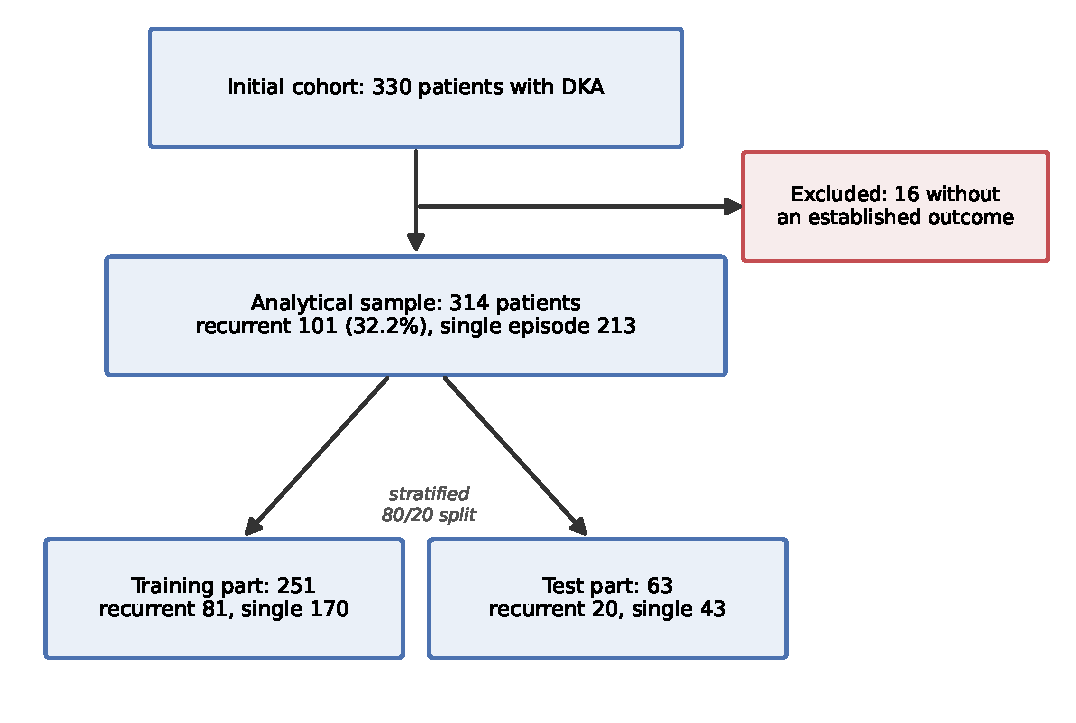
\includegraphics[width=0.55\textwidth]{flow.pdf}
\caption{Patient flow: formation of the analytical sample and the split.}\label{figflow}
\end{figure}

\begin{figure}[h]%
\centering
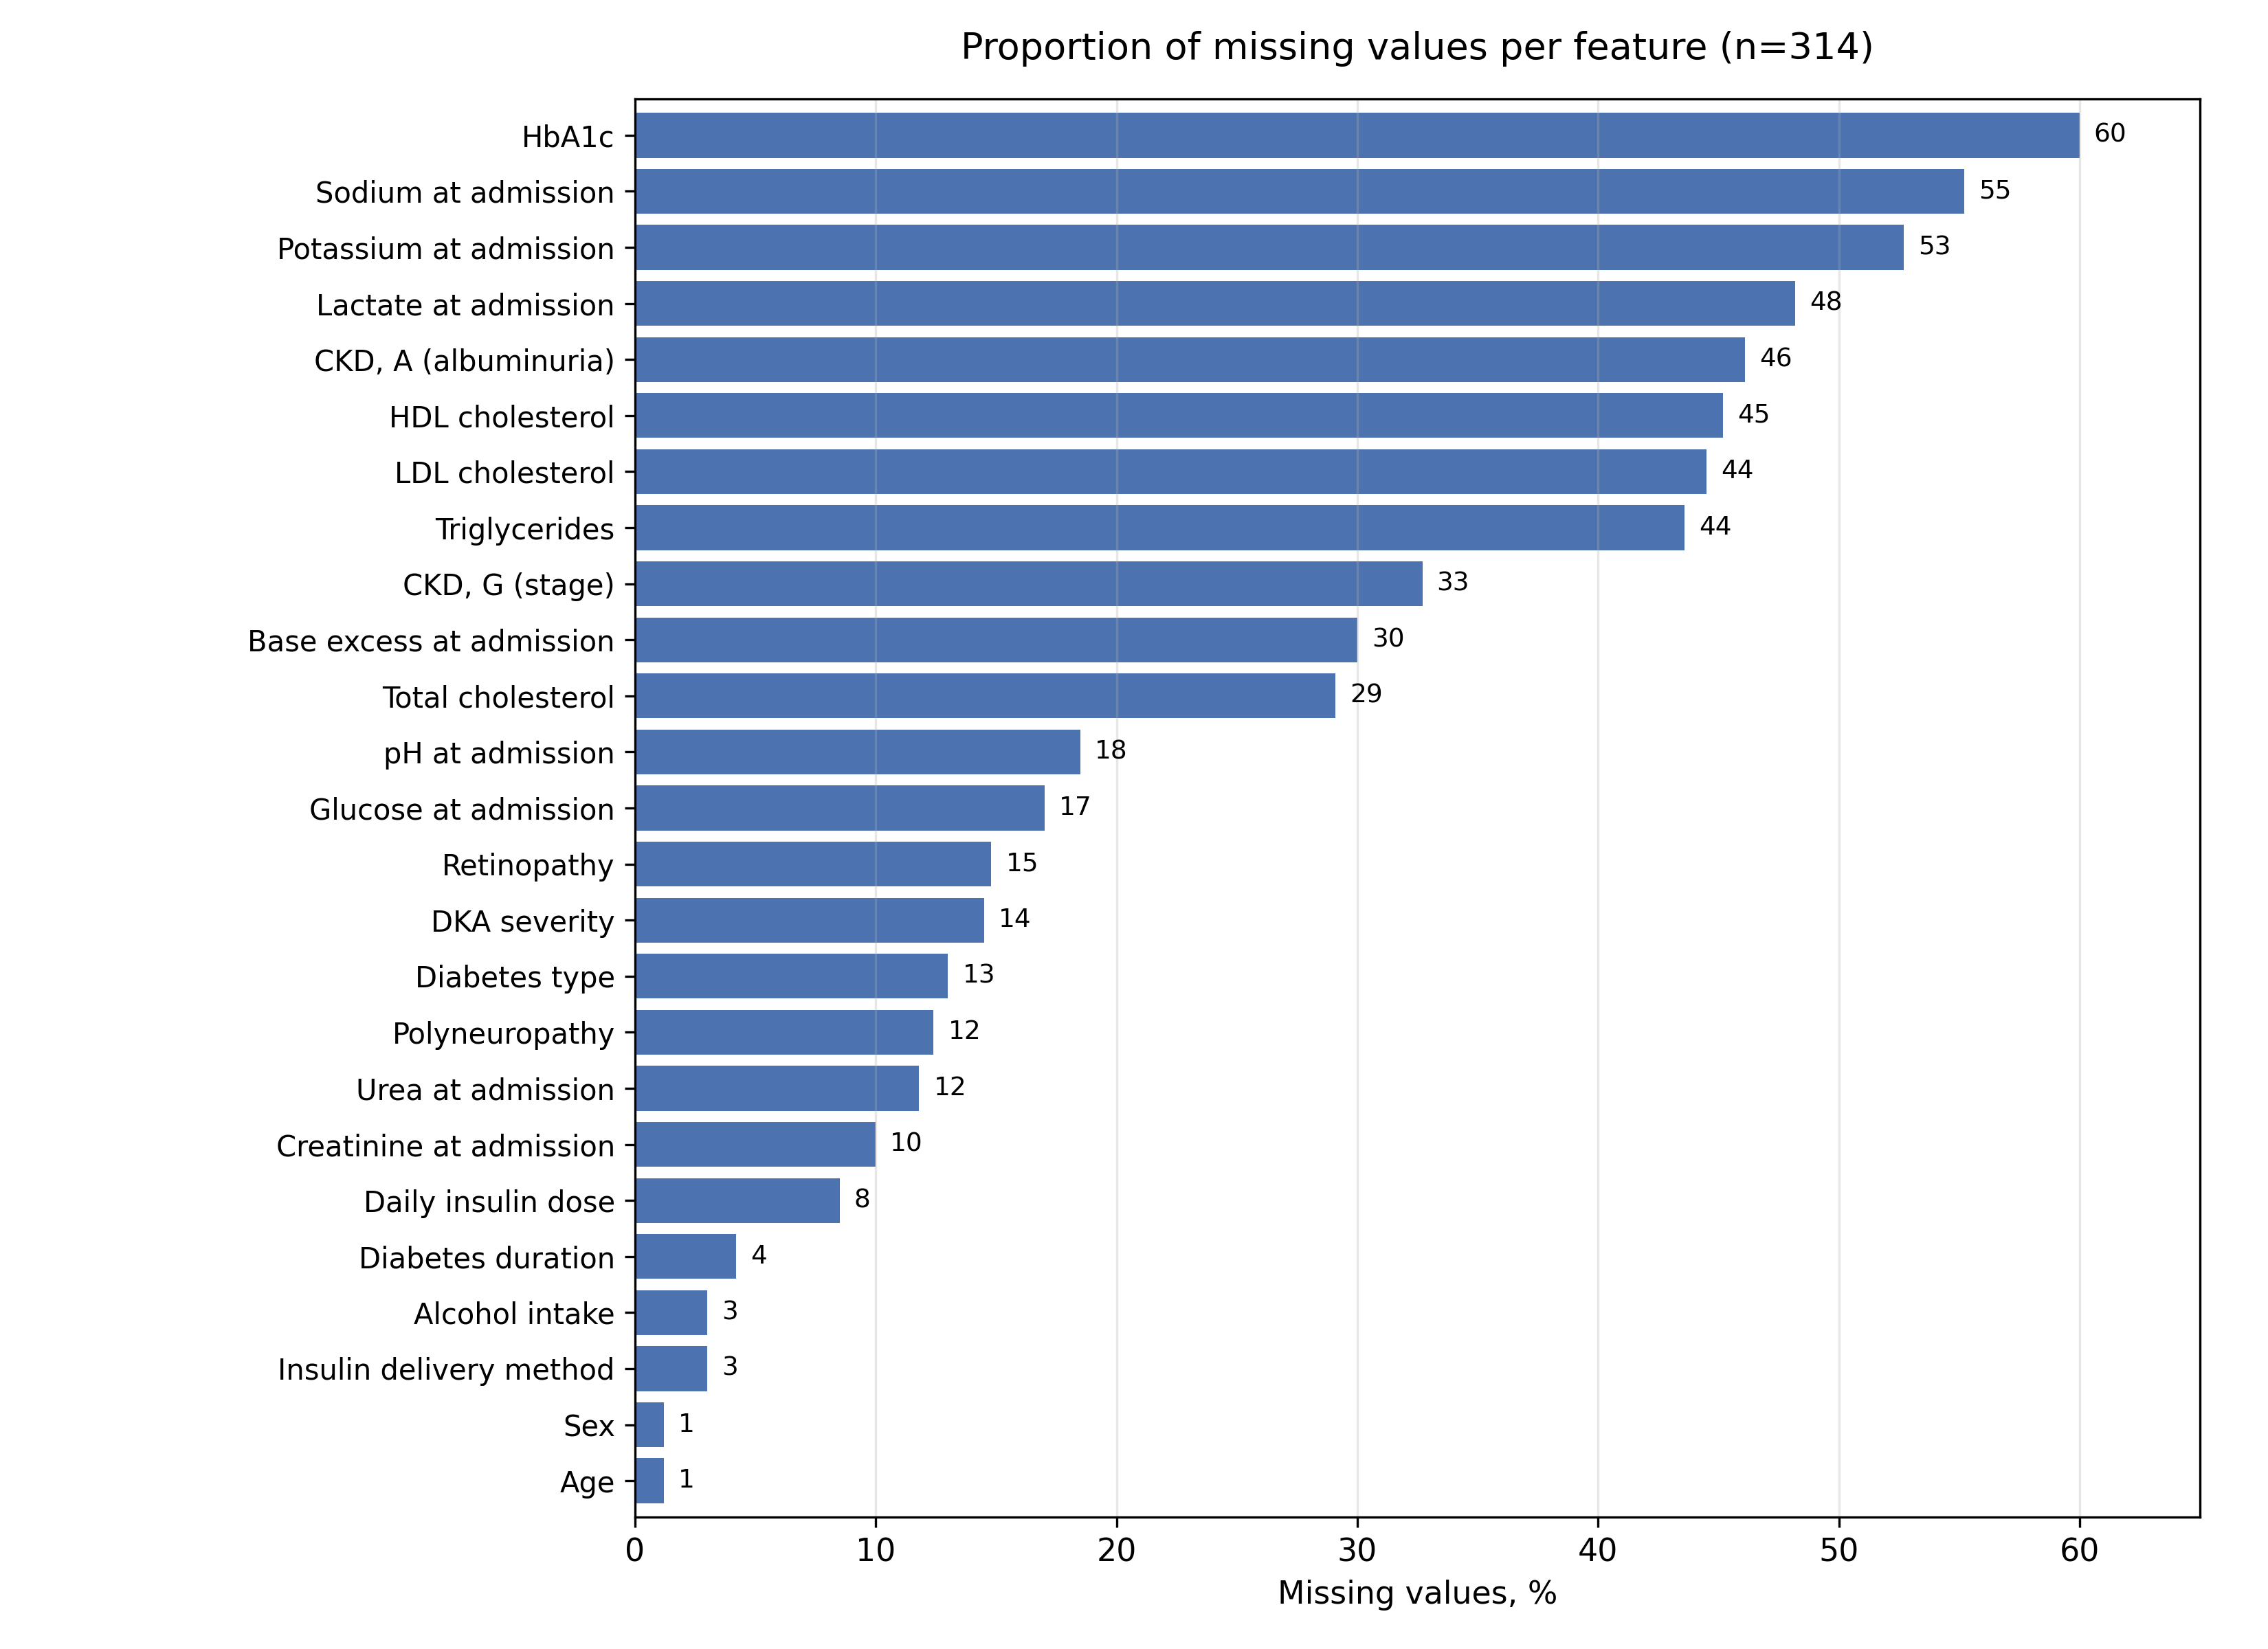
\includegraphics[width=0.75\textwidth]{fig_missingness_314.png}
\caption{Proportion of missing values per feature (n=314).}\label{figmiss}
\end{figure}

Table~\ref{tab1} collects the indicators with a significant between-group difference after the Benjamini-Hochberg correction, 10 in total.

\begin{table}[h]
\caption{Features with a significant between-group difference (Benjamini-Hochberg correction, q below 0.05)}\label{tab1}%
\begin{tabular}{@{}lllll@{}}
\toprule
Indicator & Single (n=213) & Recurrent (n=101) & q & OR (95\% CI)\\
\midrule
Daily insulin dose, units & 33 [0; 46] & 44 [35.5; 54] & $<$0.0001 & -\\
No insulin therapy, \% & 28.5 & 1.0 & $<$0.0001 & -\\
HDL cholesterol, mmol/L & 1.03 [0.83; 1.35] & 1.26 [1.03; 1.58] & 0.0020 & -\\
Diabetes duration, years & 6.75 [0; 12] & 9 [4; 15] & 0.0104 & -\\
No kidney damage (G0), \% & 60.4 & 31.1 & 0.0104 & -\\
No albuminuria (A0), \% & 56.2 & 30.6 & 0.0104 & -\\
HbA1c, \% & 12.16 (2.20) & 11.01 (2.34) & 0.0234 & -\\
No retinopathy, \% & 65.2 & 49.5 & 0.0234 & -\\
Polyneuropathy, \% & 52.5 & 68.1 & 0.0366 & 1.93 [1.15; 3.26]\\
Alcohol intake, \% & 16.2 & 28.0 & 0.0393 & 2.01 [1.14; 3.56]\\
\botrule
\end{tabular}
\footnotetext{Quantitative indicators are given as median [Q1; Q3], HbA1c as mean (standard deviation), since on this sample its distribution did not depart from normality. For categorical indicators the proportion of the stated level among known values in the group is given, missing values are not included in the denominator. The odds ratio is computed only for binary indicators.}
\end{table}

For the insulin delivery method, the main difference is driven not by the proportion on pump therapy but by the proportion of patients on no insulin therapy, 28.5\% in the single-episode group against 1.0\% in the recurrent group. This reflects a structural signal of disease onset, since a first episode by definition cannot be assigned to a recurrent course. The univariate odds ratios for features with a defined effect measure are shown in Fig.~\ref{figforest}.

\begin{figure}[h]%
\centering
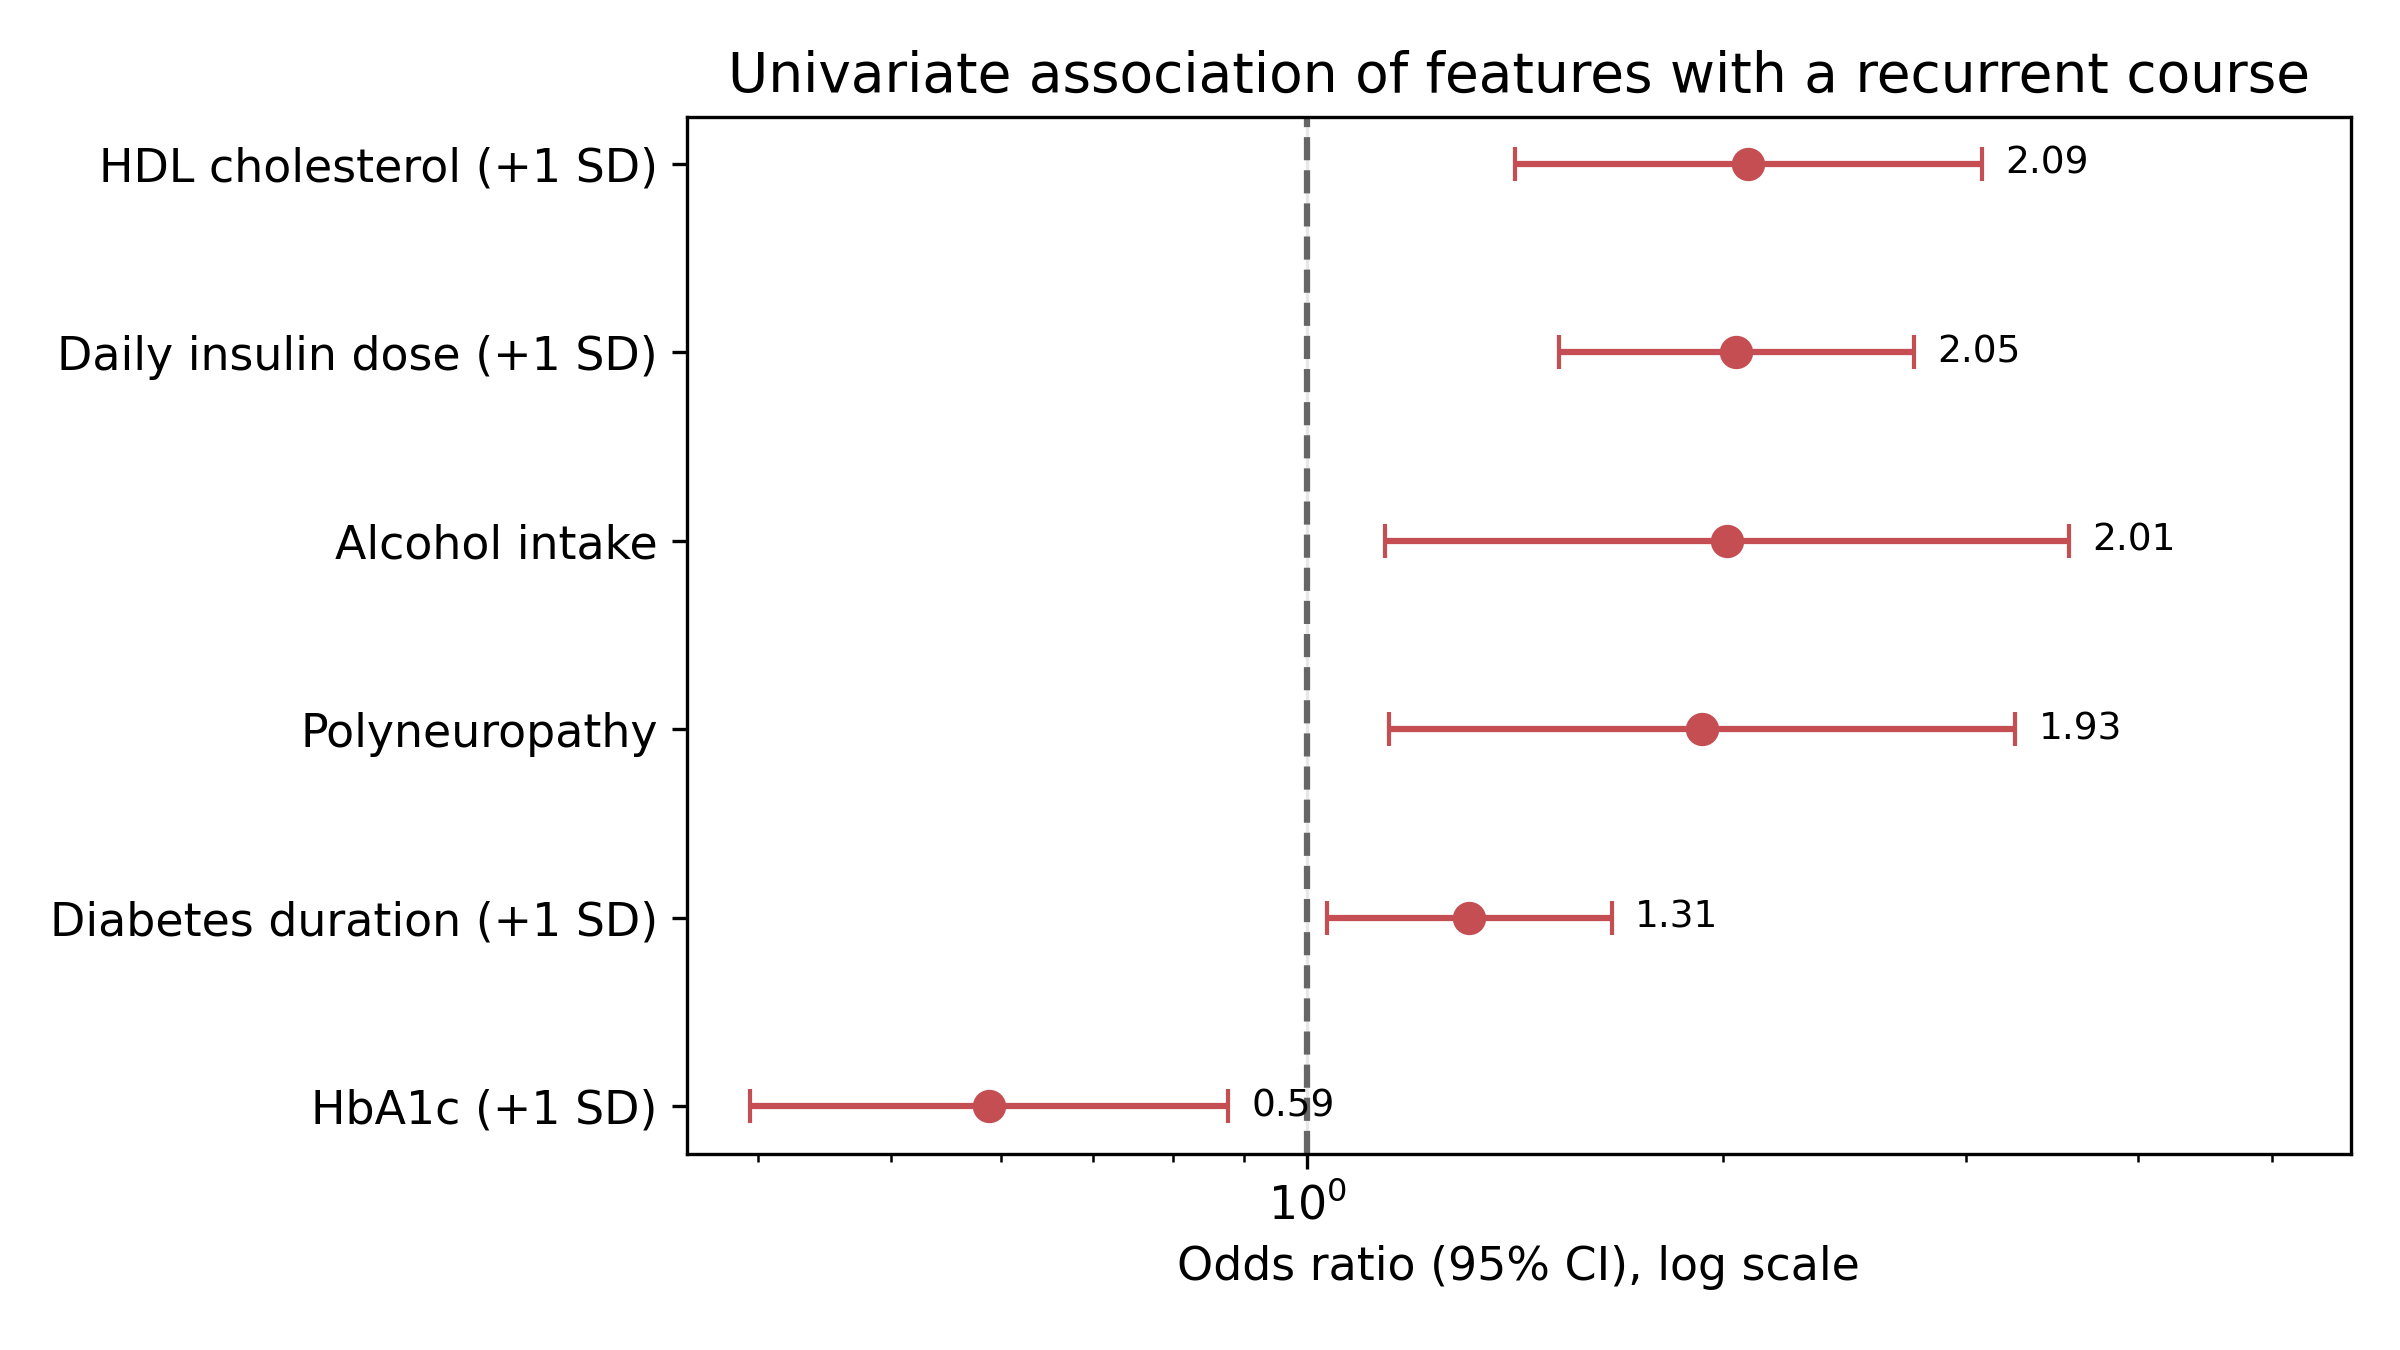
\includegraphics[width=0.8\textwidth]{fig_forest_or_314.png}
\caption{Univariate association of features with a recurrent course: odds ratios with 95\% confidence intervals.}\label{figforest}
\end{figure}

\subsection{Clinical Hypothesis: Alcohol Intake}\label{subsec3_2}

The feature value is known for 310 of 314 patients. Among patients with a recurrent course, 28.0\% (28 of 100) had consumed alcohol in the day before the episode, against 16.2\% (34 of 210) in the single-episode group. The minimum expected frequency in the 2$\times$2 table equals 20.0, so by protocol the Pearson chi-square test was applied, statistic 5.90 at one degree of freedom, p = 0.015. We reject the null hypothesis. The odds ratio was 2.01 (95\% CI 1.14-3.56), that is, alcohol intake the day before roughly doubles the odds of a recurrent course. The confidence interval reflects the precision of this estimate, it does not cover unity, which agrees with the rejection of the null hypothesis, but it remains wide and its lower bound is close to 1, so the effect size is judged with caution and the true increase in odds may be more modest than twofold. After the Benjamini-Hochberg correction the association retains significance (q = 0.039). The direction of the effect agrees with the literature \cite{ref7,ref9,ref16}.

\subsection{Discrimination}\label{subsec3_3}

\begin{table}[h]
\caption{Discrimination by nested cross-validation}\label{tab2}%
\begin{tabular}{@{}lll@{}}
\toprule
Model & ROC-AUC & SD\\
\midrule
XGBoost & 0.731 & 0.057\\
Random forest & 0.720 & 0.037\\
LightGBM & 0.719 & 0.044\\
CatBoost & 0.713 & 0.031\\
Logistic regression & 0.666 & 0.037\\
\botrule
\end{tabular}
\footnotetext{SD is the standard deviation across the outer folds of nested cross-validation.}
\end{table}

\begin{table}[h]
\caption{Discrimination on the held-out test}\label{tab3}%
\begin{tabular}{@{}ll@{}}
\toprule
Model & ROC-AUC (95\% CI)\\
\midrule
CatBoost & 0.760 [0.643; 0.867]\\
LightGBM & 0.757 [0.636; 0.867]\\
XGBoost & 0.757 [0.631; 0.873]\\
Random forest & 0.709 [0.591; 0.829]\\
Logistic regression & 0.647 [0.504; 0.782]\\
\botrule
\end{tabular}
\footnotetext{Confidence intervals were obtained by bootstrap (2000 replicates).}
\end{table}

Discrimination is given in Tables~\ref{tab2} and~\ref{tab3} and in Fig.~\ref{figroc}. Test estimates lie in the range 0.65-0.76, and nested cross-validation estimates in the range 0.67-0.73. The ranking by the two estimates agrees, the gradient boosting variants occupy the top on both cross-validation and the test, while logistic regression is below all by both estimates (0.666 and 0.647). The confidence intervals on the test are wide, about 0.24 in width on average, and overlap strongly, so the point advantage of boosting is not statistically confirmed. PR-AUC on the training part holds in the range 0.51-0.53 against a random classifier baseline of about 0.32.

\begin{figure}[h]%
\centering
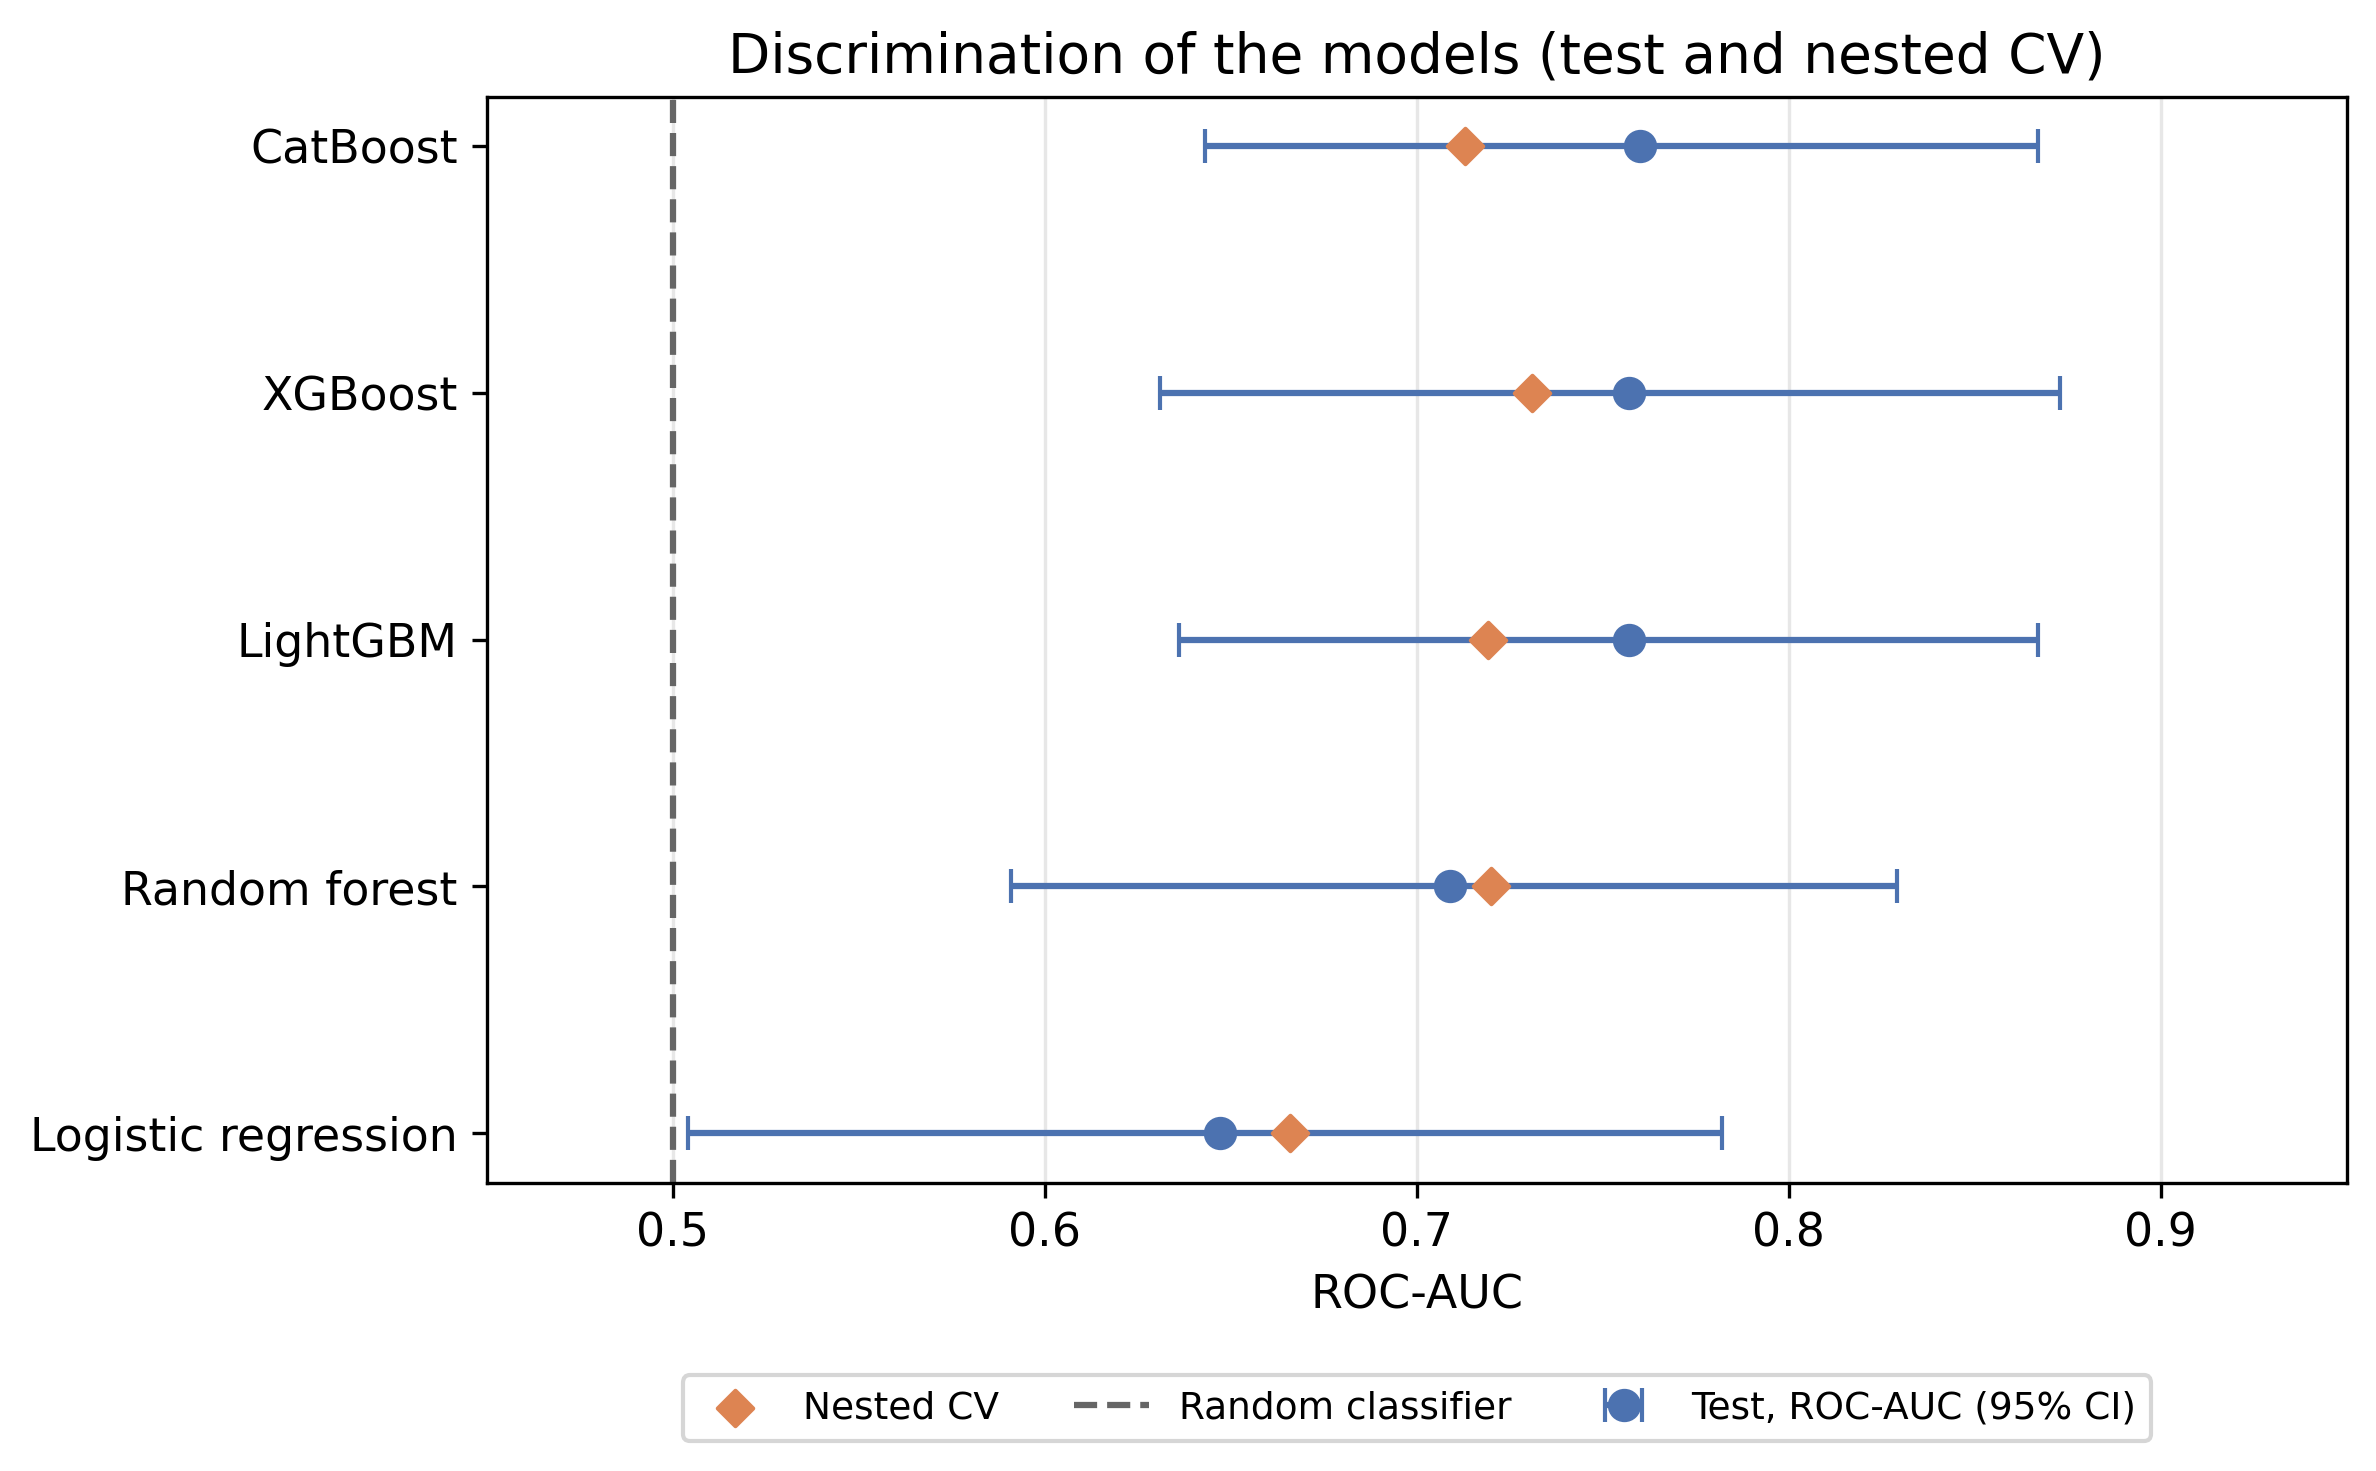
\includegraphics[width=0.8\textwidth]{fig_roc_auc_314.png}
\caption{Discrimination of the models on the held-out test (with 95\% confidence intervals) and by nested cross-validation.}\label{figroc}
\end{figure}

As a sign of overfitting we considered a systematic excess of the estimates obtained on the training part over the estimate on the held-out test beyond the 95\% confidence intervals. There is no such excess, for all five models the nested cross-validation estimate falls within the confidence interval of the test estimate. In addition, for the random forest two resampling schemes on the training part agree, the out-of-bag estimate 0.682 [0.614; 0.748] and the out-of-fold estimate 0.728 [0.662; 0.787] mutually cover each other with their confidence intervals.

Pairwise comparison of the five models by the DeLong test with the Benjamini-Hochberg correction over 10 comparisons revealed no significant pair either on the out-of-fold training part or on the held-out test. The smallest p values after correction were obtained on the test when comparing logistic regression with the boosting variants (about 0.21), where logistic regression is lower. This does not prove the superiority of boosting, since at this sample size the power of the test is low, but neither is there ground to prefer logistic regression.

\subsection{Error Structure}\label{subsec3_4}

The error structure on the held-out test at the Youden-index cut-off point is given in Table~\ref{tab4}.

\begin{table}[h]
\caption{Confusion matrix on the held-out test, Youden-index cut-off point}\label{tab4}%
\begin{tabular}{@{}llllllll@{}}
\toprule
Model & Threshold & TP & FP & FN & TN & Sens. & Spec.\\
\midrule
Random forest & 0.285 & 17 & 19 & 3 & 24 & 0.850 & 0.558\\
XGBoost & 0.385 & 16 & 18 & 4 & 25 & 0.800 & 0.581\\
CatBoost & 0.330 & 16 & 17 & 4 & 26 & 0.800 & 0.605\\
LightGBM & 0.175 & 14 & 15 & 6 & 28 & 0.700 & 0.651\\
Logistic regression & 0.240 & 12 & 18 & 8 & 25 & 0.600 & 0.581\\
\botrule
\end{tabular}
\footnotetext{Test part, 20 patients with a recurrent course and 43 with a single episode. FP is a type I error, FN is a type II error.}
\end{table}

The matrix shows what is not visible from the ROC-AUC, at similar discrimination the models distribute errors between the two types differently. At the Youden point sensitivity lies in the range 0.60-0.85 and specificity 0.56-0.65. All models catch the larger part of recurrences at the cost of a noticeable share of false alarms, from 15 to 19 of the 43 single-episode patients. Logistic regression catches the fewest, 12 recurrences of 20, the random forest the most, 17 of 20, while XGBoost and CatBoost give a close intermediate picture, 16 of 20 each. The thresholds differ markedly between models (0.18-0.39) and are unstable at this sample size, so substantive conclusions are built on ROC-AUC and PR-AUC, and the threshold is given as an illustration.

\subsection{Negative Results}\label{subsec3_5}

Transformations of quantitative features can affect only the scale-sensitive logistic regression. We compared on it the manual clinical transformation and the Yeo-Johnson transformation against standardization, the ROC-AUC hardly differed (0.699-0.700), so standardization was retained in all models. Stacking with logistic regression as the meta-model over the out-of-fold predictions of the base models gave the best combination with ROC-AUC 0.743 on the training part, which coincides with the best single model (CatBoost, 0.743). On the held-out test the best stacks gave 0.723-0.734 and did not exceed the best single model (0.760). Synthetic balancing also gave no gain. ROC-AUC for the synthetic methods was 0.699-0.714 (SMOTENC 0.699, ADASYN 0.710, SMOTE over one-hot 0.712, BorderlineSMOTE 0.714), whereas without synthetics it was 0.721-0.723. PR-AUC for synthetics is lower (0.525-0.556 against 0.573) and the Brier score higher (0.194-0.202 against 0.189), that is, calibration worsens. Synthetic generation of examples improved neither the ranking nor the calibration, so imbalance was handled by class weighting.

\subsection{Feature Importance}\label{subsec3_6}

The full feature rankings by mean absolute SHAP value agree between the four tree models and diverge from logistic regression (Fig.~\ref{figspearman}). Random forest, XGBoost, LightGBM and CatBoost correlate pairwise by Spearman at 0.62-0.91, whereas logistic regression correlates with them weakly, on average 0.26. The four tree models place the same profile at the top of the lists, daily insulin dose, HbA1c, diabetes duration and insulin delivery method. Logistic regression brings forward renal complications, the stage of CKD and albuminuria, while the insulin delivery method remains shared across all five models.

\begin{figure}[h]%
\centering
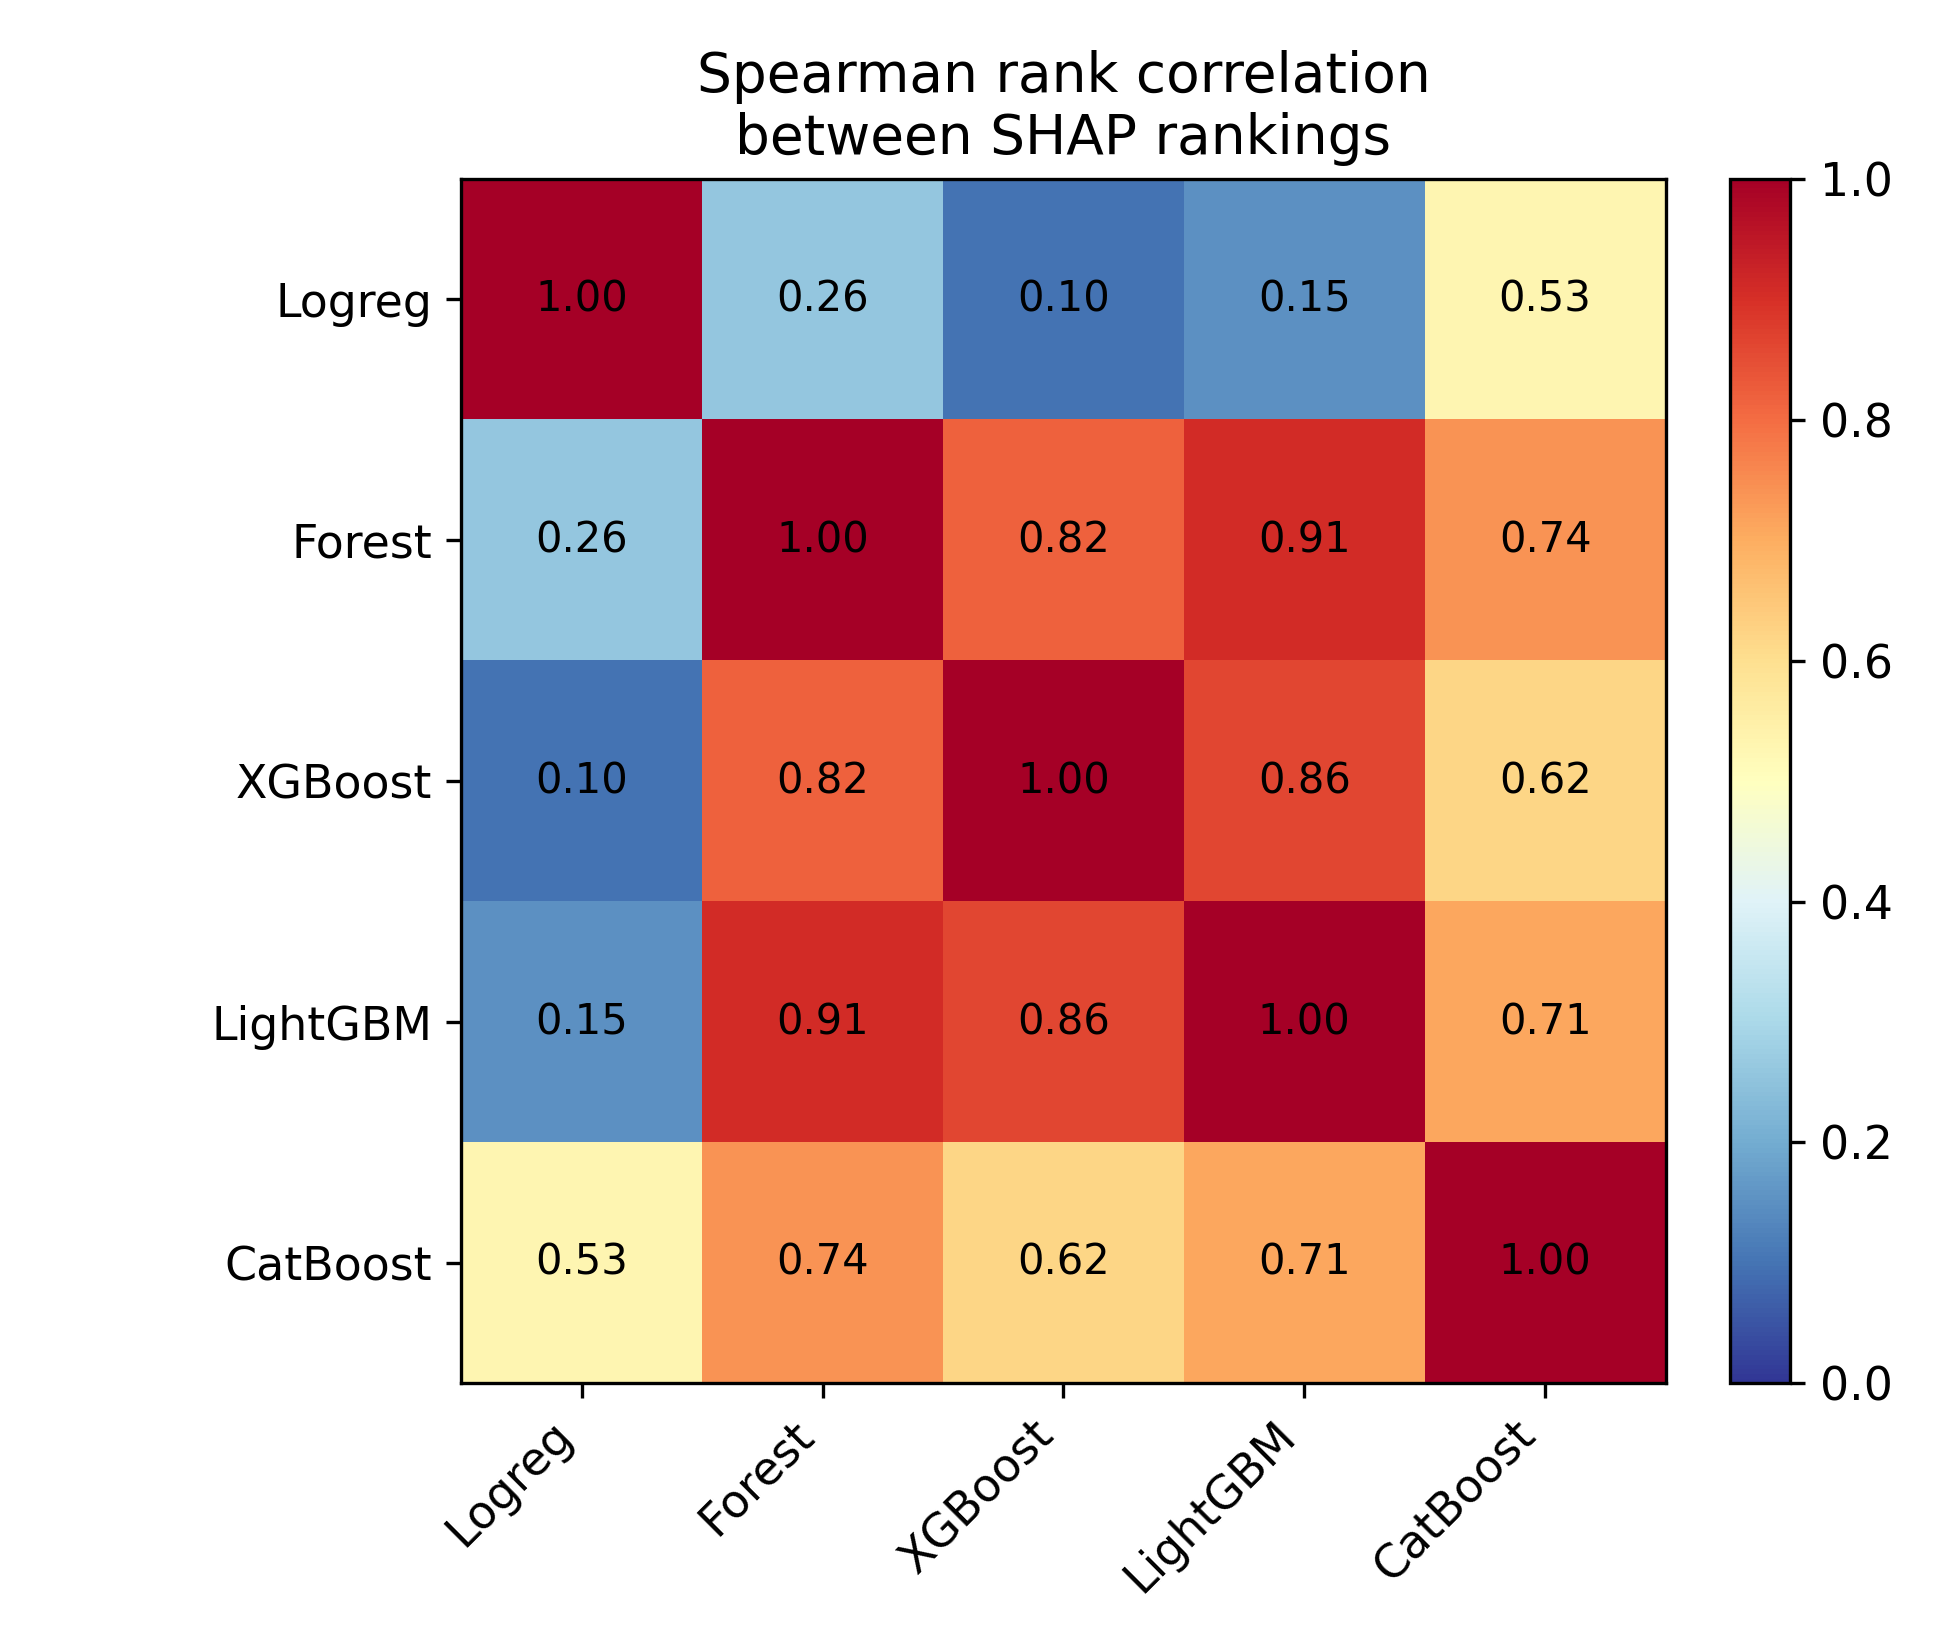
\includegraphics[width=0.6\textwidth]{fig_shap_spearman_314.png}
\caption{Pairwise Spearman rank correlation between the SHAP rankings of the models.}\label{figspearman}
\end{figure}

\begin{figure}[h]%
\centering
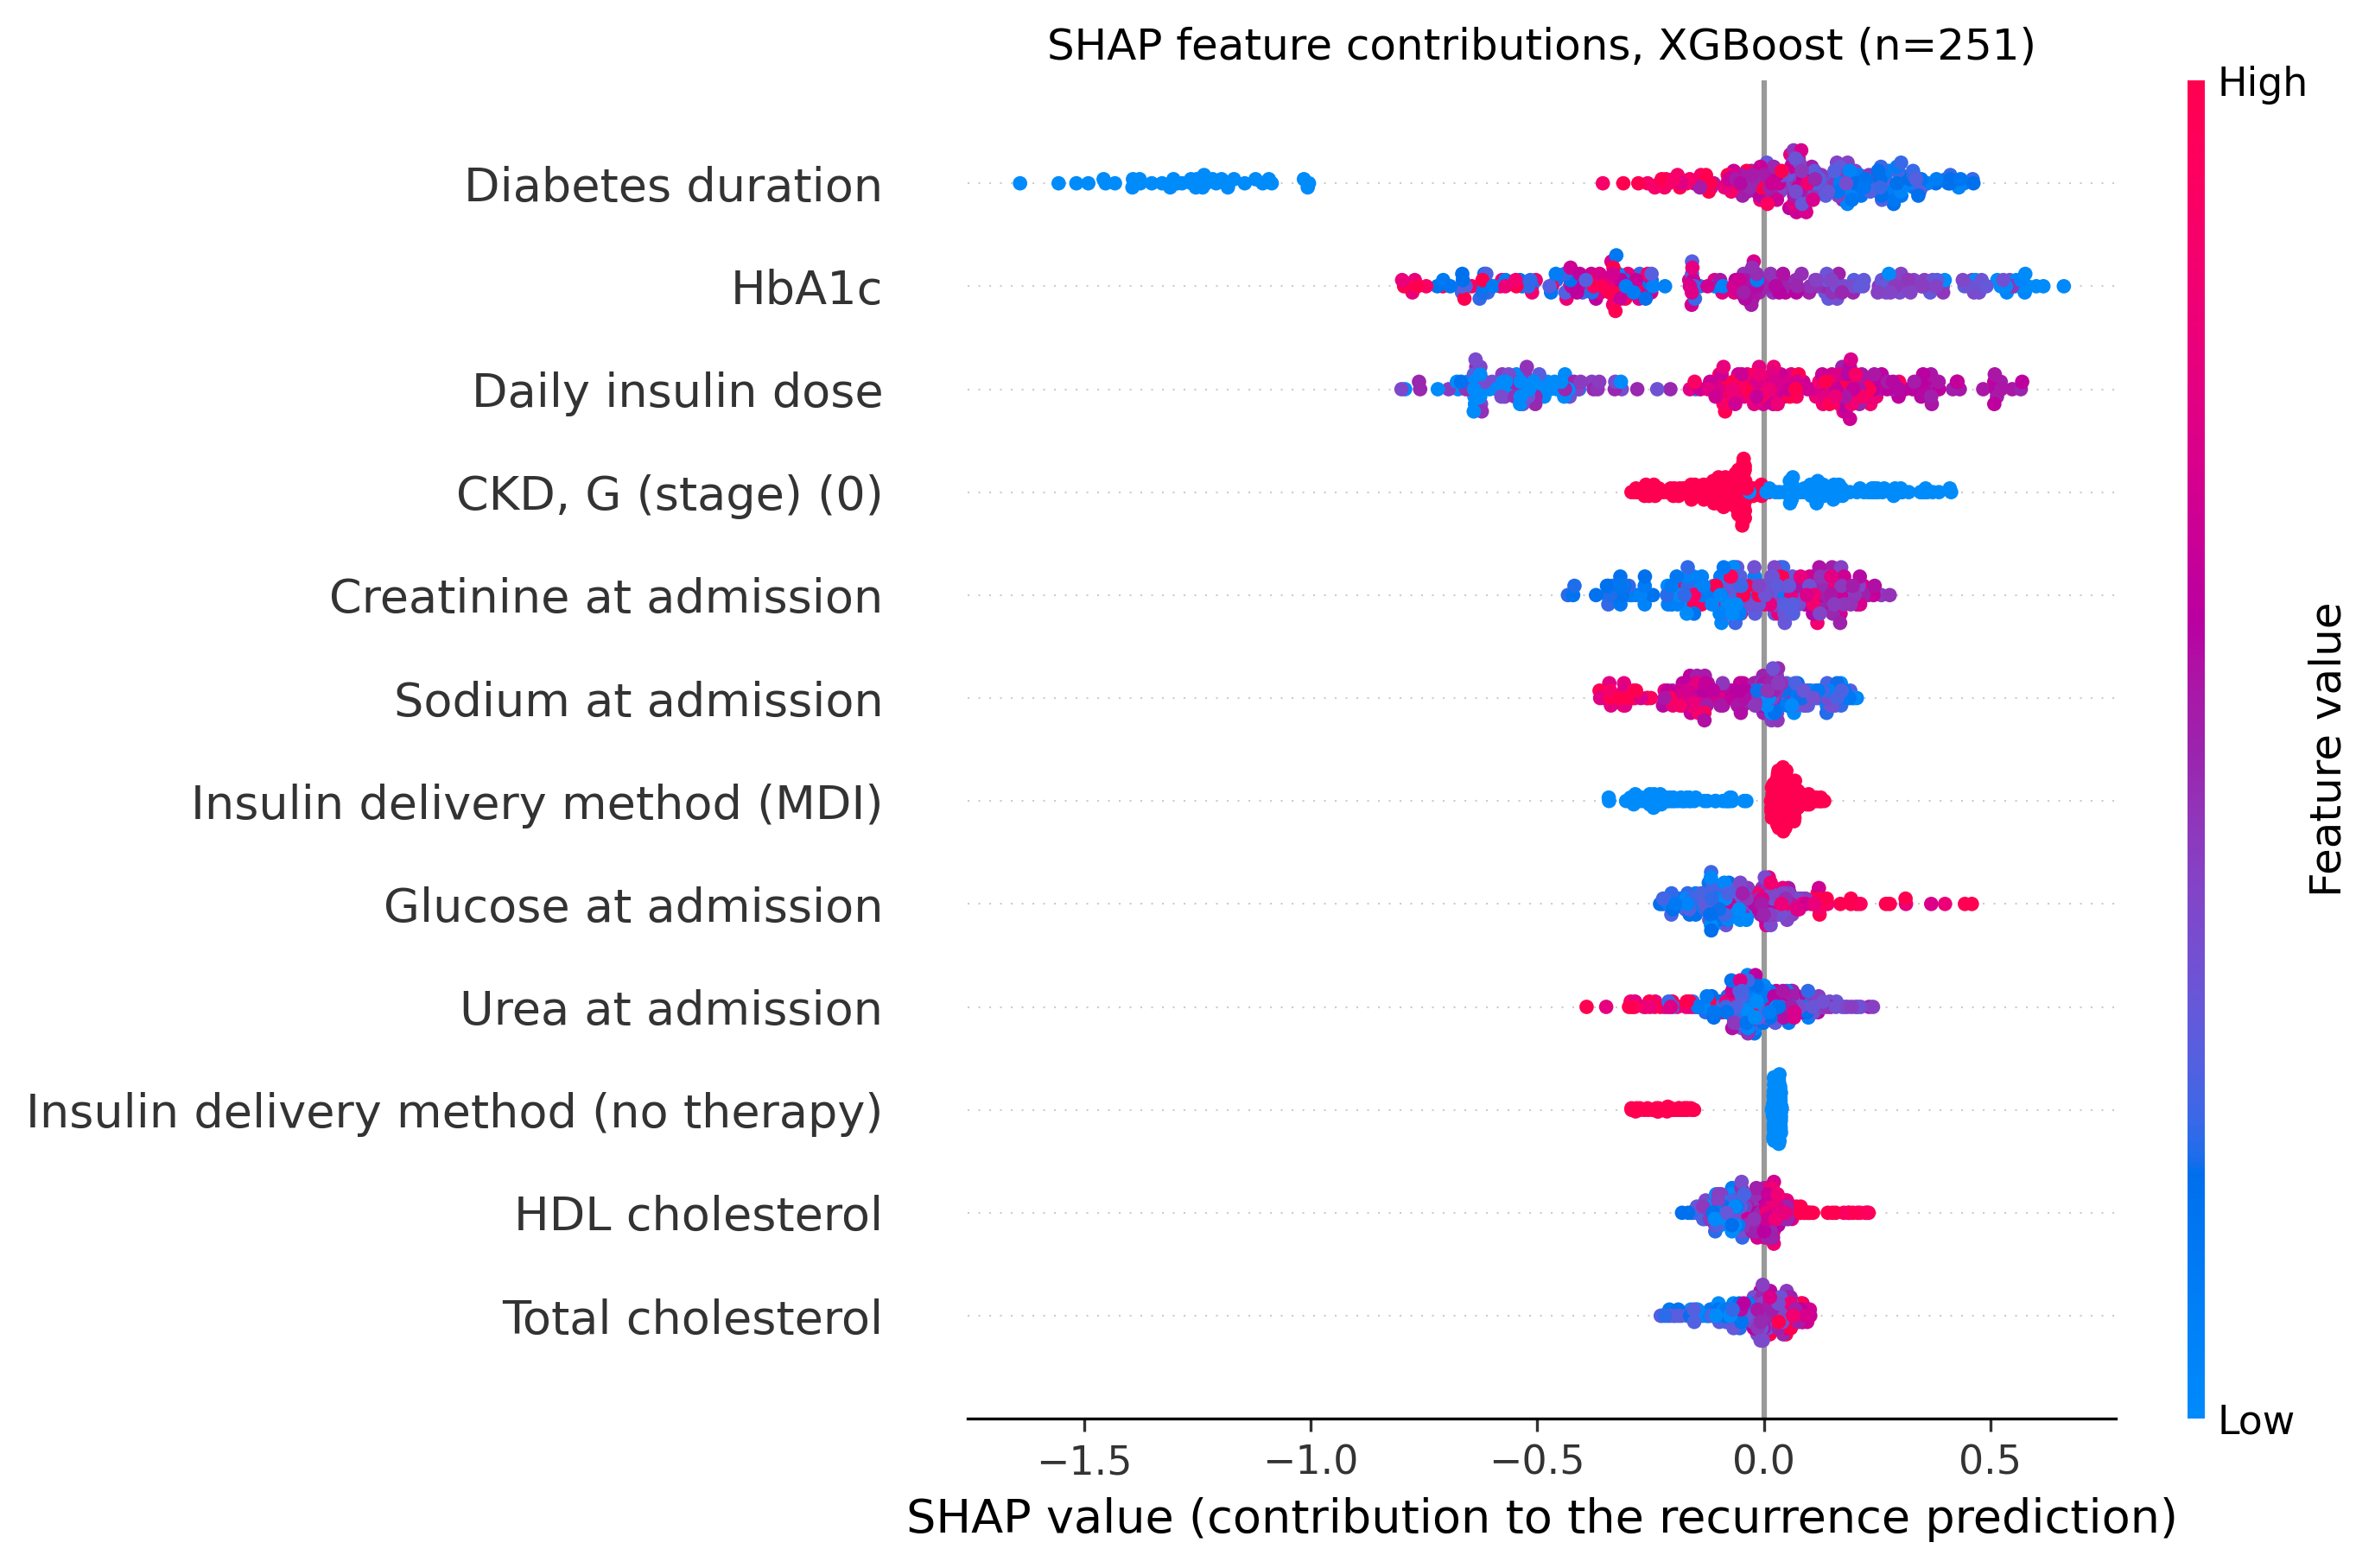
\includegraphics[width=0.8\textwidth]{fig_shap_beeswarm_xgb_314.png}
\caption{SHAP feature contributions for the leading model XGBoost.}\label{figshap}
\end{figure}

The three gradient boosting variants consistently place eight features in the top-10 by SHAP, insulin delivery method, HbA1c, HDL cholesterol, the stage of CKD, daily insulin dose, diabetes duration, creatinine and sodium at admission. The random forest, another tree ensemble, gives the same ranking (rank correlation with the boosting models 0.74-0.91) and confirms this set within the tree models. Logistic regression, a model of a different class, places the listed features lower and instead raises albuminuria, retinopathy and polyneuropathy. The set of leading features therefore depends on the model class, the tree models give one view, the linear model another. The feature contributions for the leading model XGBoost are shown in Fig.~\ref{figshap}.

The stability of the rankings to the sample composition was checked by bootstrap of the training part (200 replicates). The most stable features in the tree models are the daily insulin dose and HbA1c, which enter the top-10 of each model in 91-98\% and 86-92\% of replicates. Insulin delivery method and diabetes duration enter less often and with a wide spread across models (67-100\% and 65-90\%). The next tier, HDL cholesterol, creatinine, glucose, sodium at admission and the stage of CKD, holds in 40-67\% of replicates and is less stable. Logistic regression ranks differently, it keeps the daily insulin dose in the top-10 in only 10\% of replicates against 91-98\% in the tree models.

Comparison with classical statistics shows a partial correspondence (Table~\ref{tab5}). The four features shared across the top-10 of all models are also significant in the between-group comparison, insulin delivery method, HDL cholesterol, the stage of CKD and HbA1c. Lower down the lists the two approaches diverge. Some indicators significant in the between-group comparison contribute little by SHAP, among the tree models retinopathy enters the top-10 in only one, albuminuria and polyneuropathy in none, they are raised only by logistic regression, and alcohol intake enters the top-10 in no model. Conversely, glucose, creatinine and sodium at admission, which showed no significant between-group difference, enter the top-10 in three or four tree models.

\begin{table}[h]
\caption{Correspondence between significance in the between-group comparison and SHAP contribution}\label{tab5}%
\begin{tabular}{@{}lll@{}}
\toprule
Indicator & q & \shortstack{Tree models (of 4)\\with feature in top-10 SHAP}\\
\midrule
Insulin delivery method & $<$0.0001 & 4\\
HDL cholesterol & 0.0020 & 4\\
Kidney damage (CKD, G) & 0.0104 & 4\\
HbA1c & 0.0234 & 4\\
Daily insulin dose & $<$0.0001 & 4\\
Diabetes duration & 0.0104 & 4\\
Glucose at admission & not significant & 3\\
Creatinine at admission & not significant & 4\\
Sodium at admission & not significant & 4\\
Retinopathy & 0.0234 & 1\\
Albuminuria (CKD, A) & 0.0104 & 0\\
Polyneuropathy & 0.0366 & 0\\
Alcohol intake & 0.0393 & 0\\
\botrule
\end{tabular}
\footnotetext{Shown are indicators significant in the between-group comparison and indicators that entered the top-10 by SHAP in at least three tree models. The count is over the four tree models (random forest and three gradient boosting variants), logistic regression is excluded from the count as a model of a different class. The q value is taken from Table~\ref{tab1}.}
\end{table}

The discrepancies are expected, since the two quantities measure different things. The between-group test evaluates an isolated difference in a single indicator, whereas SHAP is the feature's contribution within a multivariate model, adjusted for the rest. Alcohol intake is illustrative, significant in the univariate comparison (OR 2.01), in the presence of the other features it contributes little and does not reach the SHAP top.

\section{Discussion}\label{sec4}

We assessed how far a patient's clinical profile at admission can distinguish a recurrent course of DKA from a single episode, and identified the factors associated with the outcome. Discrimination is moderate, ROC-AUC 0.67-0.73 by nested cross-validation and 0.65-0.76 on the held-out test, the gradient boosting variants are above logistic regression in point estimates, but the differences lie within the confidence intervals.

A recurrent course is associated with the profile of long-standing insulin-dependent diabetes, a longer disease duration, a higher daily insulin dose, and renal and microvascular complications. HbA1c is lower in the recurrent group (11.0\% against 12.2\%). Four features enter the top-10 by SHAP in all models and are at the same time significant in the between-group comparison, insulin delivery method, HbA1c, HDL cholesterol and the stage of CKD. Here the agreement of the two approaches ends, lower down the lists they diverge, as do the models of different classes.

The direction of the HbA1c difference deserves separate comment. In the recurrent group the mean HbA1c is lower, 11.0\% against 12.2\%, which contradicts the expectation that recurrences are linked to worse chronic glycemic control. A possible explanation agrees with the rest of the recurrent group's profile, a longer diabetes duration and a higher daily insulin dose, these are patients with long-standing, actively managed disease in whom an episode is more often triggered by acute causes, missed insulin or alcohol intake, rather than by sustained decompensation. The difference is moderate and its interpretation should be refined on a larger sample.

The importance of features on this sample partly depends on the choice of model. Gradient boosting, the leading family, and the closely related random forest consistently raise the metabolic profile, daily insulin dose, HbA1c and diabetes duration, but their agreement is expected, all are tree ensembles with a close construction. Logistic regression, a model of a different class, brings forward renal and microvascular complications. There is no single set of leading features independent of the algorithm on these data, and this is itself a result, on a small sample the interpretation is sensitive to the model family, so reliance on a single model is risky.

The divergence of SHAP and univariate statistics is regular, since they measure different things. Glucose, creatinine and sodium at admission entered the top-10 in three or four tree models, although on their own they do not separate the groups, the multivariate model uses them in combination with other features. The reverse case is alcohol intake, significant in the univariate comparison (OR 2.01) but, in the presence of the other features, contributing little and not reaching the SHAP top.

The clinical hypothesis was confirmed, alcohol intake in the day before an episode is associated with a recurrent course, odds ratio 2.01 (95\% CI 1.14-3.56). This carries a risk factor known from the literature over to the Russian population \cite{ref7,ref9,ref16}. The design is cross-sectional, so this concerns an association rather than a proven causation.

No model outperformed the others in discrimination, the DeLong test with correction revealed no significant difference in any of the ten pairs, either on cross-validation or on the test. In point estimates gradient boosting is above logistic regression by both estimates, so XGBoost was chosen as the working model, but at this sample size the power of DeLong is low and superiority cannot be considered proven. Stacking and synthetic balancing brought no gain. The absence of a clear leader agrees with a systematic review \cite{ref17}, where on other clinical tasks machine learning likewise did not outperform logistic regression.

A direct comparison of discrimination with published models is incorrect, since they address a different task. On a cohort of adults with type 1 diabetes a ROC-AUC of about 0.82 was obtained \cite{ref11}, up to 0.85 on a cohort of children \cite{ref10}, but both works predict the first episode or hospitalization within a set time window on large foreign databases.

\section{Limitations}\label{sec5}

The main limitation is the design. The outcome was ascertained retrospectively, so at the time the predictors were measured it had in most cases already occurred. The model is diagnostic, it does not predict a future event but separates already formed groups by clinical profile.

Diabetes duration differed between groups, a median of 9 years [4; 15] in the recurrent course against 6.75 [0; 12] in the single episode (q = 0.0104). This difference may reflect not risk but the very definition of the outcome, the longer the disease lasts, the longer the period over which a repeat episode could be recorded, and the data contain no observation interval common to all patients. Building a prognostic model requires a prospective cohort with episode dates, observation time and censoring.

The overlap of leading features across models is partial. In the tree models the daily insulin dose and HbA1c are stable (86-98\% of bootstrap replicates in each model), but the next tier, HDL cholesterol, creatinine, glucose, sodium at admission and the stage of CKD, enters the top-10 in only 40-67\% of replicates, and these features should be regarded as requiring confirmation. Logistic regression ranks these features differently. The frequencies obtained are an upper bound, the hyperparameters were fixed under resampling, and the variability of their tuning is not built into the estimate. Resampling from a single cohort, moreover, says nothing about reproducibility on data from another center.

The contribution of the insulin delivery method requires cautious interpretation. The category of no insulin therapy in our cohort almost coincides with disease onset, 28.5\% in the single-episode group against 1.0\% in the recurrent group, and a first episode by definition belongs to a single course. The high contribution of this feature therefore partly reflects the definition of the outcome rather than an independent risk. At the same time the feature is clinically meaningful and available at admission, the type of therapy at the time of DKA carries information on the stage and management of the disease. We keep it in the model but interpret its top rank in the SHAP lists with the stated reservation.

The operating point was chosen by the Youden and F2 rules on the out-of-fold predictions of the training part. At this sample size the threshold value is unstable, for Youden the confidence interval is 0.33-0.60, so the comparison of models rests on ROC-AUC and PR-AUC, and the threshold itself requires recalibration on external data before clinical use.

The remaining limitations concern the data. The sample is single-center and small, with no external validation on an independent population. The proportion of missing values in part of the laboratory indicators is high, up to 60\%, and although imputation did not appreciably distort the distributions, uncertainty remains. A number of features named in the literature as leading for a recurrent course (psychiatric disorders, treatment adherence, socioeconomic circumstances) are absent from our data, and this limits the attainable discrimination.

\section{Conclusions}\label{sec6}

A patient's clinical profile at admission separates a recurrent from a single course of DKA with moderate ability, ROC-AUC 0.67-0.73 by nested cross-validation and 0.65-0.76 on the held-out test. In the tree models (three gradient boosting variants and a random forest) the SHAP ranking is stable, the daily insulin dose and HbA1c enter the top-10 of each model in 86-98\% of bootstrap replicates, whereas logistic regression, a linear model, ranks differently and in addition raises renal and microvascular complications. Four features, insulin delivery method, HbA1c, HDL cholesterol and the stage of CKD, enter the top-10 in all models and are at the same time significant in the between-group comparison.

The clinical hypothesis was confirmed, alcohol intake in the day before an episode is associated with a recurrent course, odds ratio 2.01 (95\% CI 1.14-3.56). The superiority of any model over the others could not be demonstrated, the DeLong test revealed no significant differences, and stacking and synthetic balancing brought no gain. Gradient boosting is above logistic regression in point estimates and was therefore taken as the working model, but at this sample size this advantage is not proven.

The model is diagnostic rather than prognostic over a time horizon. A prognostic model requires a prospective cohort with episode dates and observation time, together with external validation on data from another center.

\backmatter

\bmhead{Supplementary information}

The full result tables and the SHAP figures are available in the open project repository.

\bmhead{Acknowledgements}

The authors thank the physicians who provided the de-identified clinical data.

\section*{Declarations}

\bmhead{Funding}

The study was carried out without external funding.

\bmhead{Conflict of interest}

The authors declare no conflict of interest relevant to the content of this article.

\bmhead{Ethics approval and consent to participate}

[Hospital ethics committee approval; to be filled in later.]

\bmhead{Consent for publication}

Not applicable, the work was performed on de-identified data, individual patient information is not published.

\bmhead{Data availability}

Patient data cannot be published, as this would breach confidentiality. Access is possible on reasonable request to the corresponding author within ethical constraints.

\bmhead{Materials availability}

Not applicable.

\bmhead{Code availability}

The analysis code is open and available at \url{https://github.com/ovelsad/dka-recurrence-ml}, and includes fixed library versions and instructions for reproduction.

\bmhead{Author contributions}

O. Sadykhov: study conception, data preparation and analysis, statistical analysis, model development and validation, interpretation of results, preparation of the first draft of the manuscript. V. Leonenko: study conception and design, scientific supervision, analysis methodology, verification of results, critical revision and editing of the manuscript. Both authors read and approved the final version.

\begin{thebibliography}{17}

\bibitem{ref1} Benoit, S.R., Zhang, Y., Geiss, L.S., Gregg, E.W., Albright, A.: Trends in diabetic ketoacidosis hospitalizations and in-hospital mortality - United States, 2000-2014. MMWR Morb. Mortal. Wkly. Rep. \textbf{67}(12), 362-365 (2018). \url{https://doi.org/10.15585/mmwr.mm6712a3}

\bibitem{ref2} Desai, D., Mehta, D., Mathias, P., Menon, G., Schubart, U.K.: Health care utilization and burden of diabetic ketoacidosis in the U.S. over the past decade: a nationwide analysis. Diabetes Care \textbf{41}(8), 1631-1638 (2018). \url{https://doi.org/10.2337/dc17-1379}

\bibitem{ref3} Santos, S.S., Ramaldes, L.A.L., Dualib, P.M., Gabbay, M.A.L., Sa, J.R., Dib, S.A.: Increased risk of death following recurrent ketoacidosis admissions: a Brazilian cohort study of young adults with type 1 diabetes. Diabetol. Metab. Syndr. \textbf{15}(1), 85 (2023). \url{https://doi.org/10.1186/s13098-023-01054-5}

\bibitem{ref4} Gibb, F.W., Teoh, W.L., Graham, J., Lockman, K.A.: Risk of death following admission to a UK hospital with diabetic ketoacidosis. Diabetologia \textbf{59}(10), 2082-2087 (2016). \url{https://doi.org/10.1007/s00125-016-4034-0}

\bibitem{ref5} Mohler, R., Lotharius, K., Moothedan, E., Goguen, J., Bandi, R., Beaton, R., Knecht, M., Mejia, M.C., Khoury, M., Sacca, L.: Factors contributing to diabetic ketoacidosis readmission in hospital settings in the United States: a scoping review. J. Diabetes Complications \textbf{38}(10), 108835 (2024). \url{https://doi.org/10.1016/j.jdiacomp.2024.108835}

\bibitem{ref6} Dhatariya, K.K., Glaser, N.S., Codner, E., Umpierrez, G.E.: Diabetic ketoacidosis. Nat. Rev. Dis. Primers \textbf{6}(1), 40 (2020). \url{https://doi.org/10.1038/s41572-020-0165-1}

\bibitem{ref7} Brandstaetter, E., Bartal, C., Sagy, I., Jotkowitz, A., Barski, L.: Recurrent diabetic ketoacidosis. Arch. Endocrinol. Metab. \textbf{63}(5), 531-535 (2019). \url{https://doi.org/10.20945/2359-3997000000158}

\bibitem{ref8} Kanzwl, S.M.O.S., Alhajri, A.H.M., Mohammed, Y.J.A., et al.: A comparative effectiveness of intravenous fluids and insulin regimens in the acute management of diabetic ketoacidosis (DKA) and hypoglycemia: a systematic review. Cureus \textbf{17}(10), e94902 (2025). \url{https://doi.org/10.7759/cureus.94902}

\bibitem{ref9} Cooper, H., Tekiteki, A., Khanolkar, M., Braatvedt, G.: Risk factors for recurrent admissions with diabetic ketoacidosis: a case-control observational study. Diabet. Med. \textbf{33}(4), 523-528 (2016). \url{https://doi.org/10.1111/dme.13004}

\bibitem{ref10} Williams, D.D., Ferro, D., Mullaney, C., Skrabonja, L., Barnes, M.S., Patton, S.R., Lockee, B., Tallon, E.M., Vandervelden, C.A., Schweisberger, C., Mehta, S., McDonough, R., Lind, M., D'Avolio, L., Clements, M.A.: An ``all-data-on-hand'' deep learning model to predict hospitalization for diabetic ketoacidosis in youth with type 1 diabetes: development and validation study. JMIR Diabetes \textbf{8}, e47592 (2023). \url{https://doi.org/10.2196/47592}

\bibitem{ref11} Li, L., Lee, C.C., Zhou, F.L., Molony, C., Doder, Z., Zalmover, E., Sharma, K., Juhaeri, J., Wu, C.: Performance assessment of different machine learning approaches in predicting diabetic ketoacidosis in adults with type 1 diabetes using electronic health records data. Pharmacoepidemiol. Drug Saf. \textbf{30}(5), 610-618 (2021). \url{https://doi.org/10.1002/pds.5199}

\bibitem{ref12} Rudin, C.: Stop explaining black box machine learning models for high stakes decisions and use interpretable models instead. Nat. Mach. Intell. \textbf{1}(5), 206-215 (2019). \url{https://doi.org/10.1038/s42256-019-0048-x}

\bibitem{ref13} Stiglic, G., Kocbek, P., Fijacko, N., Zitnik, M., Verbert, K., Cilar, L.: Interpretability of machine learning-based prediction models in healthcare. WIREs Data Min. Knowl. Discov. \textbf{10}(5), e1379 (2020). \url{https://doi.org/10.1002/widm.1379}

\bibitem{ref14} Ahmed, S., Kaiser, M.S., Hossain, M.S., Andersson, K.: A comparative analysis of LIME and SHAP interpreters with explainable ML-based diabetes predictions. IEEE Access \textbf{13}, 37370-37388 (2025). \url{https://doi.org/10.1109/ACCESS.2024.3422319}

\bibitem{ref15} Emi-Johnson, O.G., Nkrumah, K.J.: Predicting 30-day hospital readmission in patients with diabetes using machine learning on electronic health record data. Cureus \textbf{17}(4), e82437 (2025). \url{https://doi.org/10.7759/cureus.82437}

\bibitem{ref16} Bradford, A.L., Crider, C.C., Xu, X., Naqvi, S.H.: Predictors of recurrent hospital admission for patients presenting with diabetic ketoacidosis and hyperglycemic hyperosmolar state. J. Clin. Med. Res. \textbf{9}(1), 35-39 (2017). \url{https://doi.org/10.14740/jocmr2792w}

\bibitem{ref17} Christodoulou, E., Ma, J., Collins, G.S., Steyerberg, E.W., Verbakel, J.Y., Van Calster, B.: A systematic review shows no performance benefit of machine learning over logistic regression for clinical prediction models. J. Clin. Epidemiol. \textbf{110}, 12-22 (2019). \url{https://doi.org/10.1016/j.jclinepi.2019.02.004}

\end{thebibliography}

\end{document}
